\documentclass{article}

\usepackage{kern}

\begin{document}
    Wir verwenden unter Betrachtung einer Translalation in $C$ Richtung die Fitfunktion
    \begin{align}
        f(C + C_0,L) = \frac{1}{\sqrt{L\cdot (C + C_0)}}.
    \end{align}
    Für die spätere Bestimmung von $C_{opt}$ durch Kenntnis von $L$ und $f_L$ invertieren wir $C\mapsto f(C + C_0)$ und erhalten 
    \begin{align}
        C(f,L) = \frac{1}{\omega_L^2\cdot L} - C_0. \ref{eq:4:Capacitance}
    \end{align}

    \begin{table}[h]
        \centering
        \begin{tabular}{c|ll|ll}
             \textbf{Durchgang} & $L$ in $\si{\henry}$ & $u(L)$ in $\si{\henry}$ & $C$ in $\si{\nano\farad}$ & $u(C)$ in $\si{\nano\farad}$ \\
            \hline
            $1$ & $1.64\cdot 10^{-8}$ & $2.34\cdot 10^{-11}$ & $4.27$ & $0.02$ \\
            $2$ & $1.64\cdot 10^{-8}$ & $2.34\cdot 10^{-11}$ & $4.27$ & $0.02$ \\
            \hline
            avg. & $1.64\cdot 10^{-8}$ & $2.34\cdot 10^{-11}$ & $4.27$ & $0.02$
        \end{tabular} 
        \caption{Parameterübersicht der Funktion $f(C,L)$ für die aufgenommenen Messwerte.}
    \end{table}

    Mithilfe der durch die Kurvenanpassung erhaltenen Parameter $L$ und $C_0$ können wir unter Hinzuzug der bereits in Kapitel \ref{sec:2:LarmorBestimmungWasser} bestimmten Larmorfrequenz $f_L$ die optimale Kondensatorkapazität $C_{opt}$ bestimmen. Diese ist durch \eqref{eq:4:Capacitance} gegeben und bestimmt sich zu den Werten in Tabelle \ref{tab:4:OptimalCapacitance}.
    \begin{table}
        \centering
        \begin{tabular}{c|ll}
             & $C_{opt}$ in $\si{\nano\farad}$ & $u(C_{opt})$ in $\si{\nano\farad}$ \\
            \hline
            avg. & $10.92$ & $1.81$
        \end{tabular}
        \caption{Optimale Kondensatorkapazität $C_{opt}$ für die beiden Durchgänge gemittelt.}
        \label{tab:4:OptimalCapacitance}
    \end{table}

    \begin{figure}[h]
        \centering
        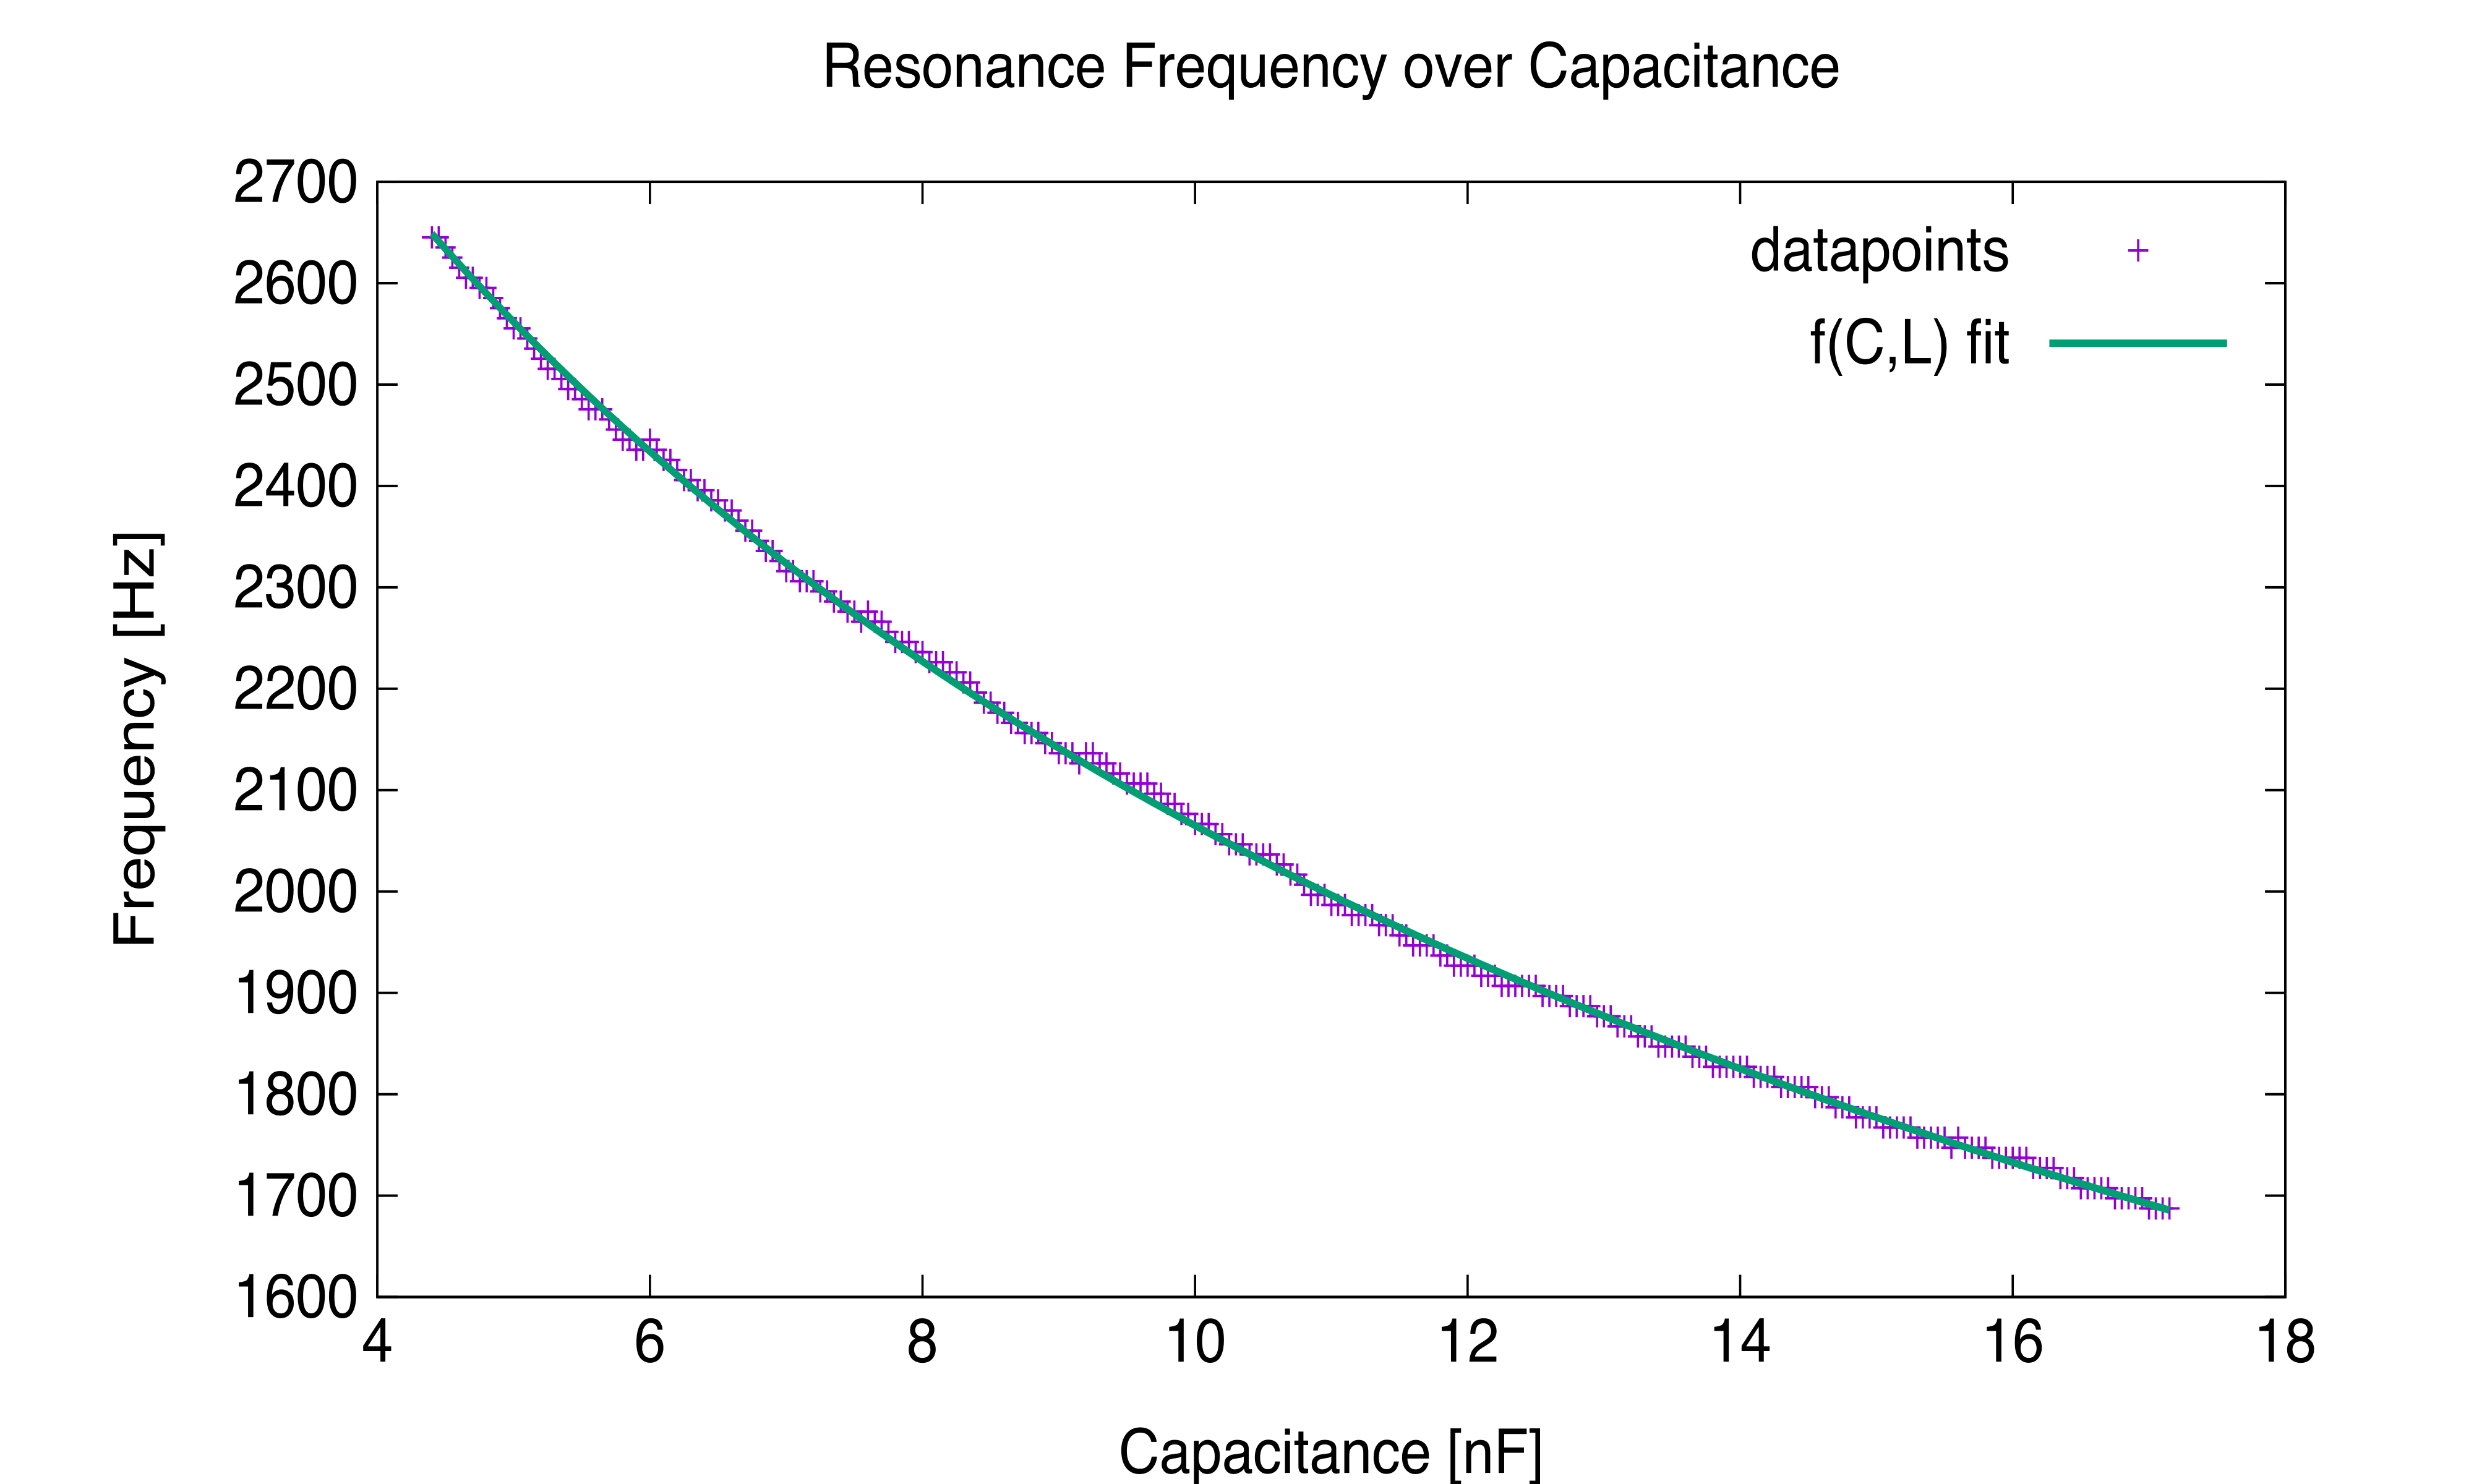
\includegraphics[width=11cm]{../Bilddateien/Messung1_Resonance_Freq_vs_Capacitance.png}
        \caption{Messung der Resonanzfrequenz in Abhängigkeit der Kapazität am Beispiel des ersten Versuchdurchgangs.}
    \end{figure}

\end{document}